% ****** Start of file apssamp.tex ******
%
%   This file is part of the APS files in the REVTeX 4.2 distribution.
%   Version 4.2a of REVTeX, December 2014
%
%   Copyright (c) 2014 The American Physical Society.
%
%   See the REVTeX 4 README file for restrictions and more information.
%
% TeX'ing this file requires that you have AMS-LaTeX 2.0 installed
% as well as the rest of the prerequisites for REVTeX 4.2
%
% See the REVTeX 4 README file
% It also requires running BibTeX. The commands are as follows:
%
%  1)  latex apssamp.tex
%  2)  bibtex apssamp
%  3)  latex apssamp.tex
%  4)  latex apssamp.tex
%
\documentclass[twocolumn,superscriptaddress,unsortedaddress,
%runinaddress,
%frontmatterverbose, 
%preprint,
%preprintnumbers,
%nofootinbib,
%nobibnotes,
%bibnotes,
 amsmath,amssymb,
 aps,
%pra,
%prb,
%rmp,
%prstab,
%prstper,
%floatfix,
]{revtex4-2}

\usepackage{graphicx}% Include figure files
\usepackage{dcolumn}% Align table columns on decimal point
\usepackage{bm}% bold math

\newcommand\abs[1]{\left|#1\right|}
\newcommand\bra[1]{\left| #1 \right \rangle}
\newcommand\ket[1]{\left \langle #1 \right |}

\begin{document}

\preprint{APS/123-QED}

\title{Coulomb interaction driven entanglement with electrons on helium}

\author{Niyaz Beysengulov}
\email{beysengu@msu.edu}
\affiliation{Department of Physics and Astronomy, Michigan State University, East Lansing, MI 48824, USA}
\author{Håkon Emil Kristiansen}
\affiliation{Department of Chemistry and Hylleraas Center for Quantum Molecular Sciences, University of Oslo, N-0316 Oslo, Norway}
\author{Øyvind Sigmundson Schøyen}
\affiliation{Department of Physics and Center for Computing in Science Education, University of Oslo, N-0316 Oslo, Norway}
\author{Zachary Stewart}
\affiliation{Department of Chemistry, Michigan State University, East Lansing, MI 48824, USA}
\author{Jared Weidman}
\affiliation{Department of Chemistry, Michigan State University, East Lansing, MI 48824, USA}
\author{Morten Hjorth-Jensen}
\affiliation{Facility for Rare Ion Beams and Department of Physics and Astronomy, Michigan State University, East Lansing, MI 48824, USA}
\affiliation{Department of Physics and Center for Computing in Science Education, University of Oslo, N-0316 Oslo, Norway}
\author{Johannes Pollanen}
\affiliation{Department of Physics and Astronomy, Michigan State University, East Lansing, MI 48824, USA}
\author{Angela Wilson}
\affiliation{Department of Chemistry, Michigan State University, East Lansing, MI 48824, USA}
\begin{abstract}
  We present bla bla
\end{abstract}

\pacs{02.70.Ss, 31.15.A-, 31.15.bw, 71.15.-m, 73.21.La}


\date{\today}% It is always \today, today,
             %  but any date may be explicitly specified


                              %display desired
\maketitle

%\tableofcontents
\section{Introduction} % Morten + Johannes + Niyaz
Entanglement is the fundamental characteristic that distinguishes
quantum systems composed of two or more coupled objects from their classical counterparts. The study of entanglement in precisely engineered quantum systems with countably many degrees of freedom is at the forefront of modern physics and is a key resource in quantum information science (QIS). This is particularly true in the development of two-qubit logic for quantum computation. Two-qubit entangling gates have been demonstrated in a wide variety of physical systems used in present-day quantum computing, including superconducting circuits~\cite{Steffen1423}, tapped ions~\cite{}, semiconductor quantum dots~\cite{Li809}, color-center defects in diamond~\cite{}, and neutral atoms in optical lattices~\cite{Saffman1010} just to name a few.




Describe problems in these systems.

Electrons on helium is another qubit platform. Here 2 qubit gates have never been discussed in a proper manner.

Coulomb interaction mediated entanglement / Forster interaction

Understanding the behavior of strongly confined electrons is of fundamental
interest for solving many-body problems.  Quantum dots, e.g. electrons
confined in semiconducting heterostructures, are of particular interest since
they exhibit, due to their small size, discrete quantum levels.  Under these
conditions, typical quantum phenomena like tunneling, entanglement and
magnetization can all be observed.   Since quantum
dots are manufactured and designed artificially at the laboratory, their
quantum levels can be arbitrarily tuned by changing the external field or the
size and shape of the system.  As a consequence, quantum dots provide a high
level of control for the dynamics and correlation of the electrons, which
makes them perfectly suited to study quantum effects in practice.  Since their
ground state shows similar shell structures and magic numbers as seen for
atoms and nuclei, these systems give the opportunity to
study electronic systems without the presence of a nucleus affecting the
electrons.  Apart from their relevance for theoretical research in quantum
physics, quantum dots offer a wide variety of applications: In particular,
their electrical and optical properties make them attractive for the use in
laser technology \cite{strauf2010,5075760} and solar cells
\cite{jenks:013111,doi:10.1021/cr900289f}, but they are also used in quantum
computers\cite{PhysRevA.57.120} and medical imaging \cite{Ben-Ari02042003}.


Our work's place in this field

%Electrons on helium represent a promising platform for investigating strongly-coupled qubits. Therefore a systematic investigation of the controlled generation of entanglement between two trapped electrons under the influence of coherent microwave driving pulses, taking into account the effects of the Coulomb interaction between electrons, is of significant importance for quantum information processing using trapped electrons.

\section{Sample, geometry considerations} % Niyaz writes this
%general information about electrons on helium
Surface state electrons (SSE) 'floating' above liquid helium originates from quantization of electron's perpendicular to the surface motion in a trapping potential formed by attractive force from image charge and a large $\sim$ 1 eV barrier at the liquid-vacuum interface. At low temperatures the SSE are trapped in the lowest Rydberg state for vertical motion some 11 nm above the helium surface, which is perfectly clean and has a permittivity close to that of vacuum. The weak interaction with enviorment, which is mainly governed by interaction with quantized surface capillary waves (ripplons) and bulk phonons, ensures long coherence times - a vital ingredient for any qubit platform. SSE's in-plane motion can be further localized by using microdevices on the length scales approaching the interelectron separation (at the order of one micron). 

\begin{figure}
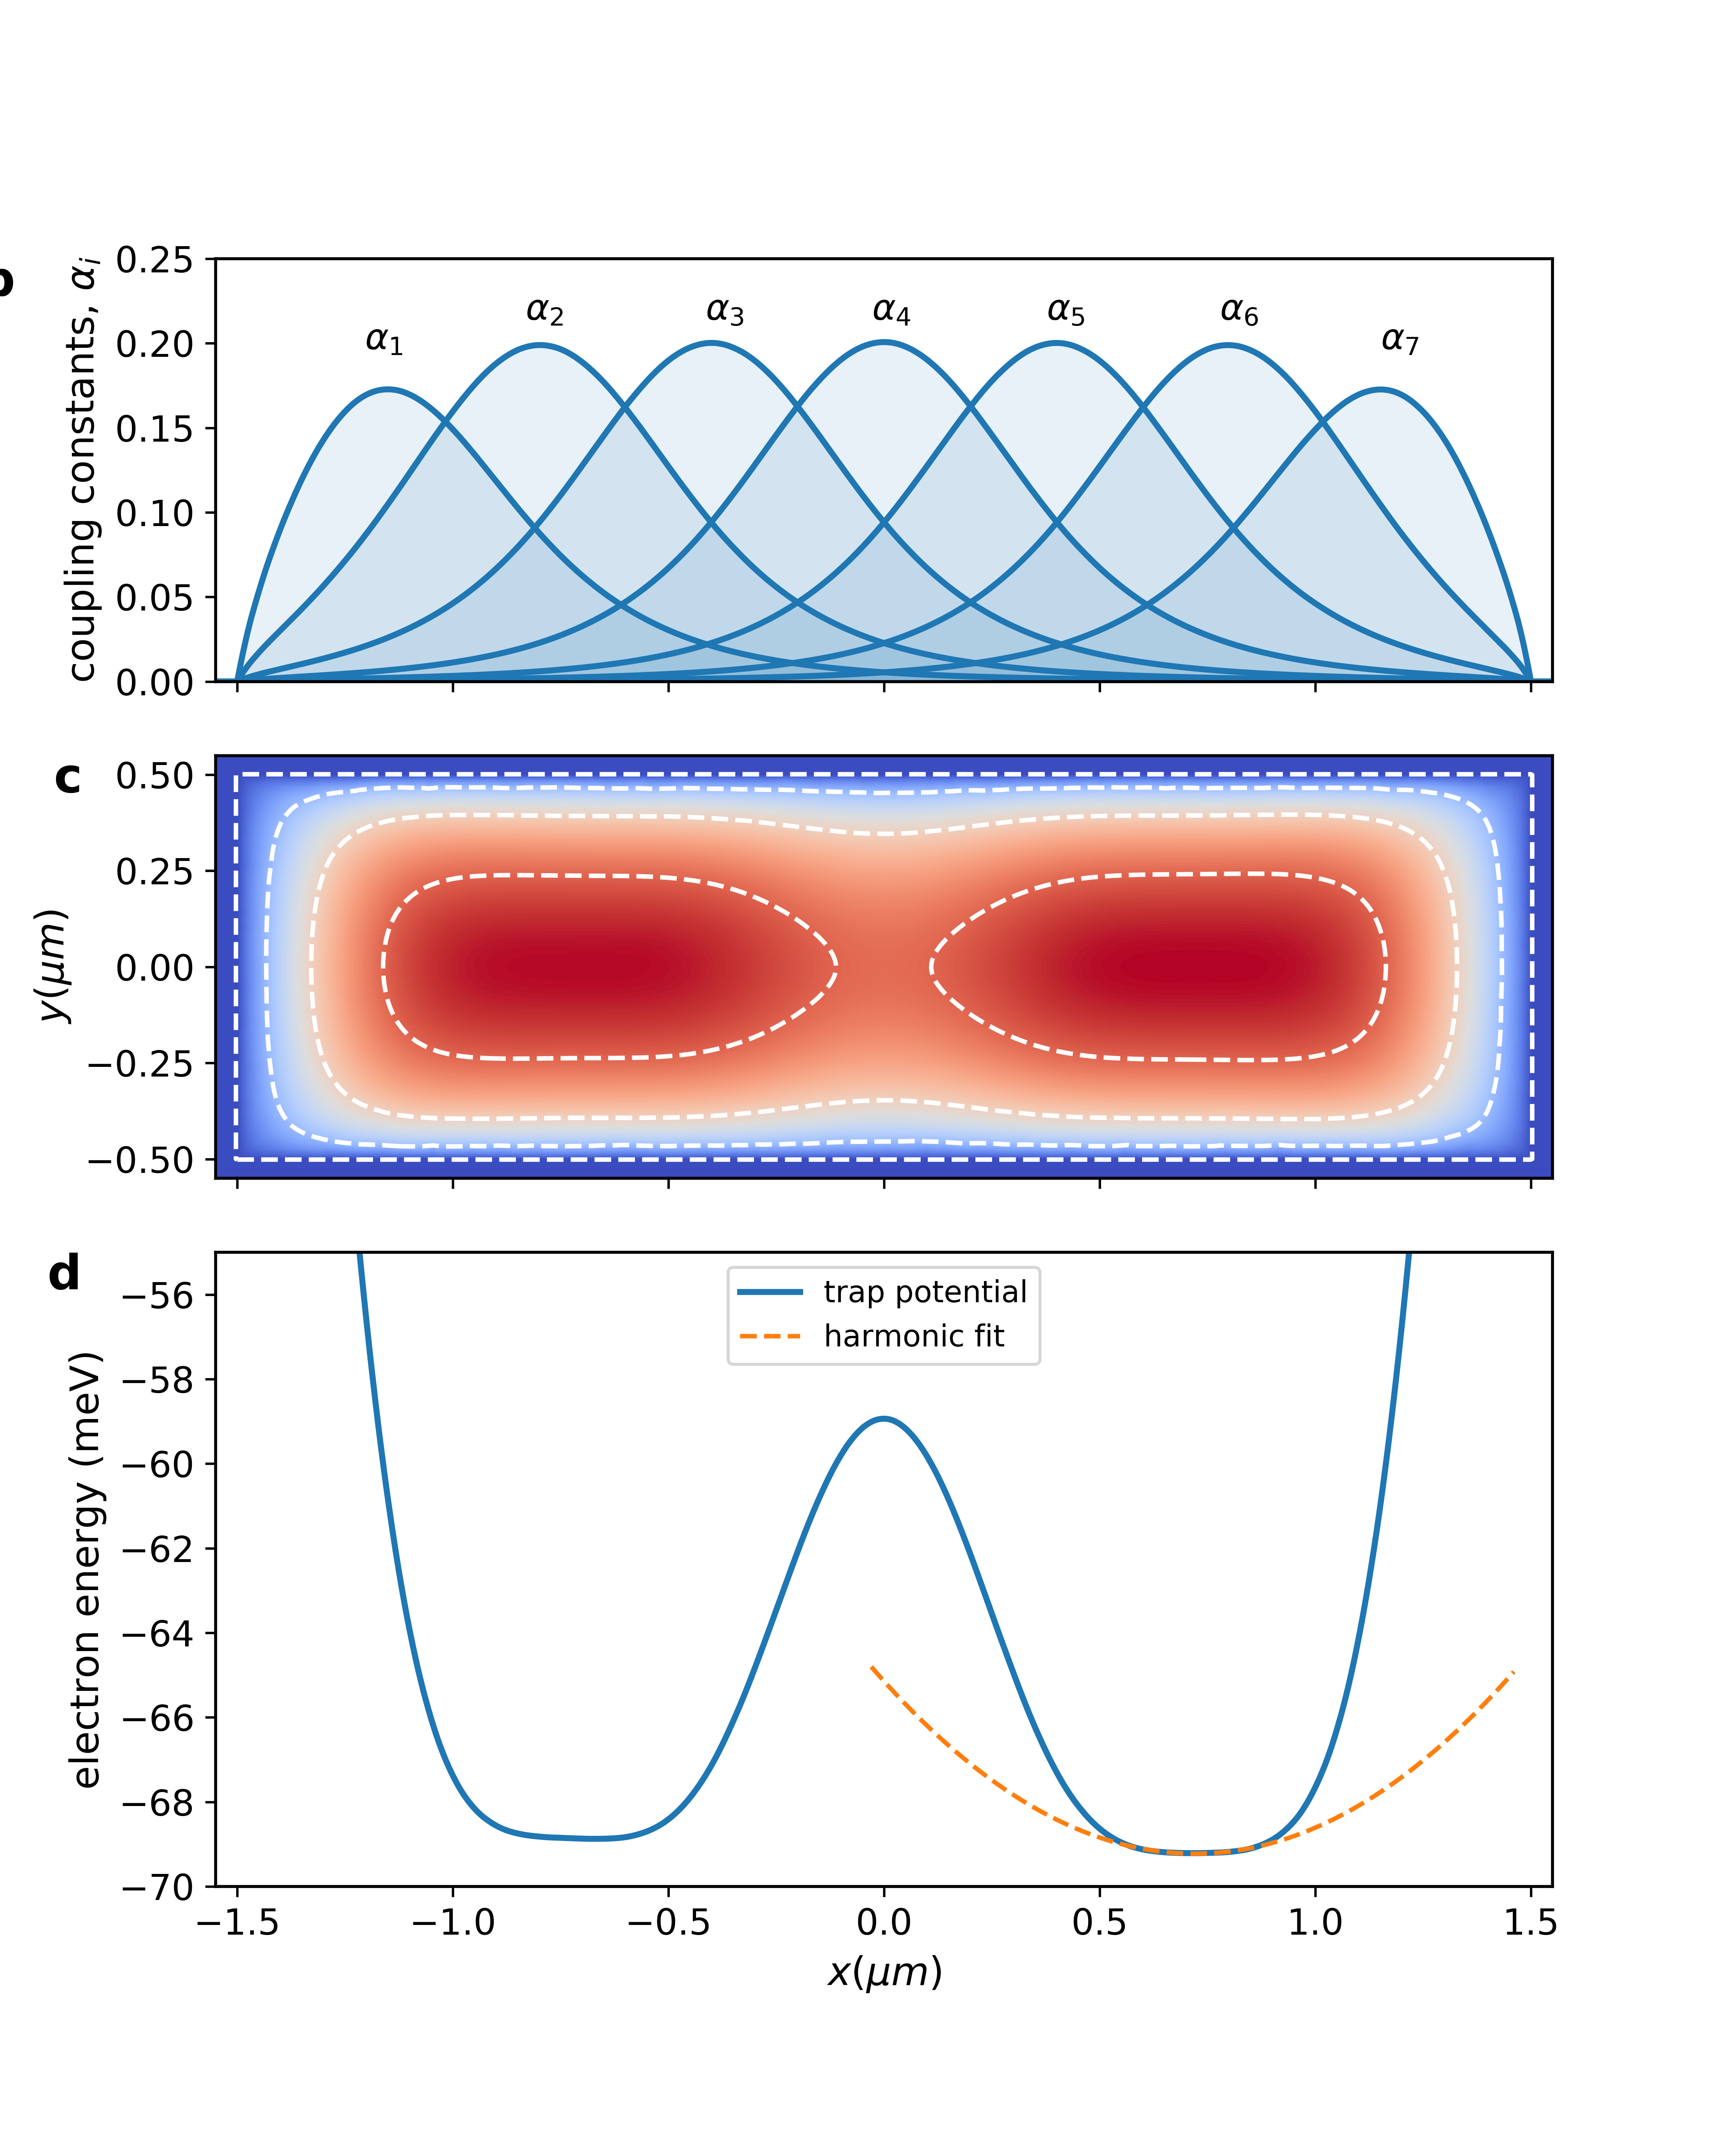
\includegraphics[width=0.49\textwidth]{Fig1.png}
\caption{\label{fig3} (a) Figure caption.}
\end{figure}

\section{Computational Methods} % Hakon, Oyvind
    As we are only studying a model comprised of two electrons restricted to move in a
    one-dimensional external potential we have employed the
    \emph{ab-initio} method configuration-interaction to compute the steady-state
    properties of the system.
    We have used a static, one-dimensional, grid-based basis set for the single-particle
    functions.
    This allows for flexibility in the choice of the external potential.

    \subsection{Finite difference basis set}
    \subsection{Full configuration-interaction method}

\section{Results and Discussion} % all of us

\section{Conclusions} % we can wait to write this one until the end

\section{\label{sec:level1}Problem: Many-level system interacting with EM field}

We start with the following problem in general form: we have a quantum-mechanical system described with Hamiltonian $H_0$ and states $\bra{n}$ being eigenfunctions of $H_0$.
\begin{equation*}
H_0 \bra{n} = E_n \bra{n}
\end{equation*}
We would like to know how these states evolve in time in the presence of a time-varying electric field. The interaction of quantum systems with electric fields is described by the Hamiltonian $ H_i = - \mathbf{E}(t) \mathbf{d}$, where $\mathbf{E}(t) = \mathbf{\mathcal{E}}_0 \cos \omega t$ and $\mathbf{d}$ is the dipole moment of the quantum system. Note, here we use dipole approximation (wavelength of the EM field is much larger than characteristic size of the quantum system wavefunction). The evolution of the quantum wavefunction is governed by Schrodinger equation:
\begin{equation}
 i \dot{\psi} = H \psi
\label{eq1}.
\end{equation}
where $H = H_0 + H_i$ (note, $\hbar = 1$). We seek the solution in the form $\psi(t) = \sum_n C_n(t) e^{-i E_n t}$. (I think something is up here... as this is a TD-CI expansion and the Slater determinants of the system should be on the right side if I am not mistaken, how should they be referred? $\Phi$?) We evolve this solution through Eq.~\ref{eq1} and get the following answer:
\begin{equation}
 i \dot{C_m} = -\frac{1}{2} \mathbf{\mathcal{E}}_0 \sum_{\alpha} \sum_{n} C_n e^{i \omega_{mn} t + i \alpha \omega t} \mathbf{d}_{mn}
\label{eq2},
\end{equation}
\begin{equation}
 \langle m\bra{n} = \delta_{mn}, \ket{m} \mathbf{d} \bra{n} = \mathbf{d}_{mn}, E_m - E_n = \omega_{mn}
\end{equation}
Here we used $\cos \omega t = \frac{1}{2} \sum_{\alpha = \pm} e^{i \alpha \omega t}$. Lets assume the system is in the ground state at $t = 0$, so $C_n(0) = \delta_{n1}$. We integrate Eq.~\ref{eq2} and get an expression:
\begin{equation}
 C_m = \frac{i}{2} \mathbf{\mathcal{E}}_0 \sum_{\alpha} \mathbf{d}_{m1} \frac{e^{i (\omega_{mn} + \alpha \omega) t} - 1}{i (\omega_{m1} + \alpha \omega)} 
\label{eq3}.
\end{equation}
An important condition here is:
\begin{equation}
\abs{\frac{\mathbf{\mathcal{E}}_0 \mathbf{d}_{m1}}{\omega_{m1} \pm \omega}} \ll 1
\label{eq4},
\end{equation}
which defines the 2-level approximation

\begin{acknowledgments}

The work of MHJ is supported by the U.S. Department of Energy, Office of Science, office of Nuclear Physics under grant No. DE-SC0021152 and U.S. National Science Foundation Grants No. PHY-1404159 and PHY-2013047. JP acknowledges support from the National Science Foundation via grant number DMR-2003815 as well as the valuable support of the Cowen Family Endowment at MSU. The work of NRB is supported by a sponsored research grant from EeroQ Corp. JP and NRB thank J.R. Lane and J.M. Kitzman for illuminating discussions.
\end{acknowledgments}
\bibliography{apssamp}% Produces the bibliography via BibTeX.

\end{document}
%
% ****** End of file apssamp.tex ******
